%\title{Modelo de Projeto de pesquisa}
%% abtex2-modelo-projeto-pesquisa.tex, v-1.9 laurocesar
%% Copyright 2012-2013 by abnTeX2 group at http://abntex2.googlecode.com/ 
%%
%% This work may be distributed and/or modified under the
%% conditions of the LaTeX Project Public License, either version 1.3
%% of this license or (at your option) any later version.
%% The latest version of this license is in
%%   http://www.latex-project.org/lppl.txt
%% and version 1.3 or later is part of all distributions of LaTeX
%% version 2005/12/01 or later.
%%
%% This work has the LPPL maintenance status `maintained'.
%% 
%% The Current Maintainer of this work is the abnTeX2 team, led
%% by Lauro César Araujo. Further information are available on 
%% http://abntex2.googlecode.com/
%%
%% This work consists of the files abntex2-modelo-projeto-pesquisa.tex
%% and abntex2-modelo-references.bib
%%

% ------------------------------------------------------------------------
% ------------------------------------------------------------------------
% abnTeX2: Modelo de Projeto de pesquisa em conformidade com 
% ABNT NBR 15287:2011 Informação e documentação - Projeto de pesquisa -
% Apresentação 
% ------------------------------------------------------------------------ 
% ------------------------------------------------------------------------

\documentclass[
	% -- opções da classe memoir --
	12pt,				% tamanho da fonte
%	openright,			% capítulos começam em pág ímpar (insere página vazia caso preciso)
	oneside,			% para impressão em verso e anverso. Oposto a oneside
	a4paper,			% tamanho do papel. 
	% -- opções da classe abntex2 --
	chapter=TITLE,		% títulos de capítulos convertidos em letras maiúsculas
	section=TITLE,		% títulos de seções convertidos em letras maiúsculas
	subsection=Title,	% títulos de subseções convertidos em letras maiúsculas
	subsubsection=Title,% títulos de subsubseções convertidos em letras maiúsculas
	% -- opções do pacote babel --
	brazil,				% o último idioma é o principal do documento
	]{abntex2}

% ---
% PACOTES
% ---

% ---
% Pacotes fundamentais 
% ---
\usepackage{lmodern}			% Usa a fonte Latin Modern
\usepackage[T1]{fontenc}		% Selecao de codigos de fonte.
\usepackage[utf8]{inputenc}		% Codificacao do documento (conversão automática dos acentos)
\usepackage{indentfirst}		% Indenta o primeiro parágrafo de cada seção.
\usepackage{color}				% Controle das cores
\usepackage{graphicx}			% Inclusão de gráficos
\usepackage{microtype} 			% para melhorias de justificação
\usepackage{amsmath}
% ---

% ---
% Pacotes adicionais, usados apenas no âmbito do Modelo Canônico do abnteX2
% ---
\usepackage{lipsum}				% para geração de dummy text
% ---

% ---
% Pacotes de citações
% ---
\usepackage[brazilian,hyperpageref]{backref}	 % Paginas com as citações na bibl
\usepackage[alf]{abntex2cite}	% Citações padrão ABNT

% --- 
% CONFIGURAÇÕES DE PACOTES
% --- 

% ---
% Configurações do pacote backref
% Usado sem a opção hyperpageref de backref
\renewcommand{\backrefpagesname}{Citado na(s) página(s):~}
% Texto padrão antes do número das páginas
\renewcommand{\backref}{}
% Define os textos da citação
\renewcommand*{\backrefalt}[4]{
	\ifcase #1 %
		Nenhuma citação no texto.%
	\or
		Citado na página #2.%
	\else
		Citado #1 vezes nas páginas #2.%
	\fi}%
% ---

% ---
% Informações de dados para CAPA e FOLHA DE ROSTO
% ---
\titulo{Poker: uma abordagem probabilística}
\autor{Universidade Estadual de Maringá -- UEM\\  Centro de Ciências Exatas\\ \vspace{2cm} André Felipe Berdusco Menezes RA:88897 \\ Victor Hugo Nagahama RA:89347 }
\local{Maringá -- Paraná}
\data{Setembro de 2015}
% O preambulo deve conter o tipo do trabalho, o objetivo, 
% o nome da instituição e a área de concentração 
\preambulo{Projeto de final de semestre apresentado como requisito parcial para obtenção de aprovação na disciplina Métodos e Técnicas de Pesquisa, no Curso de Estatísitca, na Universidade Estadual de Maringá.}
% ---

% ---
% Configurações de aparência do PDF final

% alterando o aspecto da cor azul
\definecolor{blue}{RGB}{41,5,195}

% informações do PDF
\makeatletter
\hypersetup{
	%pagebackref=true,
	pdftitle={\@title}, 
	pdfauthor={\@author},
	pdfsubject={\imprimirpreambulo},
	pdfcreator={LaTeX with abnTeX2},
	pdfkeywords={abnt}{latex}{abntex}{abntex2}{projeto de pesquisa}, 
	colorlinks=true,       		% false: boxed links; true: colored links
	linkcolor=black,          	% color of internal links
	citecolor=black,        		% color of links to bibliography
	filecolor=magenta,      		% color of file links
	urlcolor=blue,
	bookmarksdepth=4
}
\makeatother
% --- 

% --- 
% Espaçamentos entre linhas e parágrafos 
% --- 

% O tamanho do parágrafo é dado por:
\setlength{\parindent}{1.3cm}

% Controle do espaçamento entre um parágrafo e outro:
\setlength{\parskip}{0.2cm}  % tente também \onelineskip

% ---
% compila o indice
% ---
\makeindex
% ---

% ----
% Início do documento
% ----
\begin{document}

% Retira espaço extra obsoleto entre as frases.
\frenchspacing 

% ----------------------------------------------------------
% ELEMENTOS PRÉ-TEXTUAIS
% ----------------------------------------------------------
% \pretextual

% ---
% Capa
% ---
\imprimircapa
% ---

% ---
% Folha de rosto
% ---
\imprimirfolhaderosto
% ---

% ---

% NOTA DA ABNT NBR 15287:2011, p. 4:
%  ``Se exigido pela entidade, apresentar os dados curriculares do autor em
%     folha ou página distinta após a folha de rosto.''
% ---

% ---
% inserir lista de ilustrações
% ---
%\pdfbookmark[0]{\listfigurename}{lof}
%\listoffigures*
%\cleardoublepage
% ---

% ---
% inserir lista de tabelas
% ---
%\pdfbookmark[0]{\listtablename}{lot}
%\listoftables*
%\cleardoublepage
% ---

% ---
% inserir o sumario
% ---
\pdfbookmark[0]{\contentsname}{toc}
\tableofcontents*
\cleardoublepage
% ---


% ----------------------------------------------------------
% ELEMENTOS TEXTUAIS
% ----------------------------------------------------------
\textual

% ----------------------------------------------------------
% Introdução
% ----------------------------------------------------------
\chapter{Introdução}
Nos últimos anos o pôquer tornou-se um dos jogos de cartas mais praticados no mundo, devido a muito fatores, entre eles a internet. Assim sendo, julgamos importante descrever sua história, como é praticado a modalidade mais jogada e por fim transparecer a relação do jogo com a probabilidade, uma vez que, o pôquer exige um entendimento probabilístico.

Levando em conta o tema abordado e os objetivos do projeto, o presente trabalho está organizado em seu desenvolvimento da seguinte forma. Na Seção 4.1 descrevemos um breve histórico do pôquer desde da origem até os dias atuais. Na sequência, seção 4.2, explicamos a modalidade mais praticada do pôquer. Enfim, exibe-se o pôquer usando uma abordagem probabilística, em que é discutido nas seções 4.3, 4.4 e 4.5.      

% ----------------------------------------------------------
% Capitulo de textual  
% ----------------------------------------------------------
\chapter{Objetivos}

\section{Objetivo geral}
\begin{itemize}
	\item Compreender o pôquer usando uma abordagem probabilística.
\end{itemize}

\section{Objetivos específicos}
\begin{itemize}
	\item Descrever um breve histórico do pôquer e o seu desenvolvimento;
	\item Apresentar a aplicabilidade da distribuição de probabilidade hipergeométrica em uma partida de pôquer, na modalidade \textit{Texas Hold'em};
	\item Expor estratégias para tomada de decisão no \textit{Texas Hold'em} com um embasamento probabilístico.
\end{itemize}


\chapter{Metodologia}
De acordo com o problema abordado buscou-se uma metodologia de cunho bibliográfico (colocar os autores). Em um primeiro momento buscamos a compreensão da história e do entendimento do jogo de pôquer, uma vez que, este se tornou o objeto de pesquisa.

\begin{citacao}
Um bom prognóstico é probabilístico. [...] em geral, não é possível prever com exatidão o conjunto de cartas, entre as 1.326 possibilidades, que seu adversário detém até que sejam reveladas, mesmo se o oponente for habilidoso e se comportar de modo imprevisível (SILVER, 2013, p.306).
\end{citacao}     

Como pode perceber na citação acima o pôquer envolve um ``prognóstico probabilístico'' o que infere o entendimento da probabilidade, nesse sentido priorizou-se compreender e mostrar de forma clara como se calcular probabilidades no \textit{Texas Hold'em} através da distribuição discreta de probabilidade hipergeométrica. 

E por fim expor alguns conceitos usuais na tomada decisão do jogador, tais como \textit{Outs}, \textit{Odds}, \textit{Pot Odds} e a aplicação da esperança matemática. 


\chapter{Desenvolvimento}

\section{Breve histórico}
Segundo Sippets (2010) o pôquer que conhecemos hoje teve inicio nos Estados Unidos ao longo dos séculos XVII e XIX, com a chegada de imigrantes que procuravam trabalho, porém não há uma origem exata do jogo. Sabe-se que o pôquer foi influenciado por muitas civilizações, muitos atribuem seu começo com o jogo Persa ``As Nas'', no qual consistia em um baralho de 20 ou 25 cartas, além disso era similar ao pôquer aberto de cinco cartas (\textit{5 -- card stud}). 

No decorrer de sua história o pôquer recebeu muitas variações de muitos povos, no entanto conceitos básicos como estratégia, capacidade de julgamento do adversário e a classificação das cartas sempre estiveram presentes. Apesar da incerteza de sua origem, a influência americana que o pôquer sofreu pós-século XVIII foi a maior responsável por seu desenvolvimento mundial. 

Desde então o pôquer fechado (\textit{draw poker}) e o pôquer aberto de cinco cartas (\textit{5 -- card stud}) foram as variantes mais jogadas no século XX, porém essas modalidades não possuíam muita dinâmica de jogo, devido a pouca possibilidades de mãos, isto é, em tais modalidades o jogador está restrito apenas as cartas que recebiam. Contudo desenvolveu-se a modalidade \textit{Texas Hold'em} na qual os jogadores para ganhar deveriam obter a melhor combinação entre as cartas pessoais e as cartas comunitárias (da mesa). 

No ano de 2003, o número de jogadores de pôquer aumentou radicalmente e o jogo difundiu-se na televisão. A mudança foi causada principalmente por dois fatores: o desenvolvimento do pôquer \textit{online} e a vitória de um jogador amador na Série Mundial de Pôquer no torneio de \textit{Texas Hold'em}. O campeão, Chris Moneymaker, inscreveu-se inicialmente em um torneio preliminar de 40 dólares via internet, que ao fim, ocasionou a participar da série mundial, na qual foi premiado com 2,5 milhões de dólares pela vitória.

\begin{figure}[t]
	\centering
	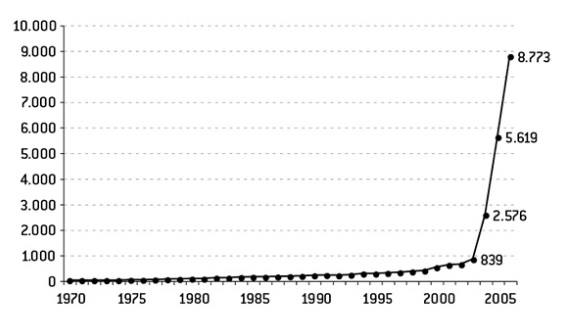
\includegraphics[scale=.7]{grafico}
	\caption{Número de participantes na Série Mundial de Pôquer entre 1970 e 2006}
	\label{participantesWSOP}
\end{figure}

\clearpage
\section{Disposições gerais sobre o \textit{Texas Hold'em}}
Dentre todas as modalidades do pôquer\footnote{Para conhecer todas as modalidades acesse: https://www.pokerstars.com/br/poker/games/}, a mais jogada é o \textit{Texas Hold'em}, conhecido como \textit{Hold'em}, a modalidade é jogada com um baralho tradicional de 52 cartas, com 4 naipes e 13 cartas de valores numéricos distintos, em que nenhum naipe é superior ao outro, e o Ás é a carta mais alta e 2 a mais baixa (Figura \ref{ordem cartas}). Outro elemento necessário para praticar o jogo são as fichas, cujo valores podem ser reais ou fictícios. O número de jogadores em um jogo competitivo varia entre dois a dez participantes.

\begin{figure}[h]
	\centering
	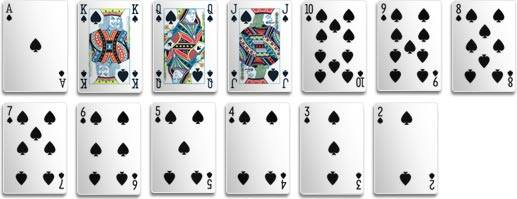
\includegraphics[scale=.6]{ordem-cartas}
	\caption{Ordem das cartas no \textit{Texas Hold'em}}
	\label{ordem cartas}
\end{figure}

Uma mão\footnote{Neste caso o termo mão se refere a cada jogo em si, normalmente com duração de alguns minutos, que vai da distribuição das cartas à sua revelação} inicia-se com o crupiê (\textit{Dealer}) distribuindo duas cartas viradas para baixo para cada jogador, na qual são chamadas de cartas pessoais. Em seguida são apresentadas cinco cartas com a face virada para cima, chamada de cartas comunitárias. Cada participante deve obter a melhor combinação entre as duas cartas pessoais e as cinco cartas comunitárias, podendo ele utilizar duas, uma ou nenhuma carta pessoal, essa combinação é determinada conforme o ranking disposto na Figura \ref{rakingmaos}.

\begin{figure}[h]
	\centering
	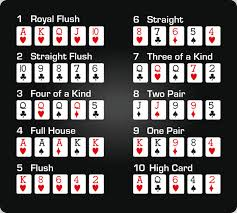
\includegraphics[scale=.84]{ranking}
	\caption{Ranking das mãos no \textit{Texas Hold'em}}
	\label{rakingmaos}
\end{figure}


No mesmo instante da distribuição das cartas o primeiro jogador a esquerda do crupiê, coloca o \textit{Small blind}, a primeira aposta obrigatória. O participante a esquerda do \textit{Small blind} paga o \textit{Big blind}, que refere-se a duas vezes o valor do \textit{Small blind}, o valor dos \textit{blinds}, isto é, as apostas são definidas previamente. Por exemplo, em um jogo \textit{Hold'em} \$10/\$20 possui um \textit{Small blind} \$10 e um \textit{Big blind} \$20. O montante das apostas é denominado pote.

Cada jogador possui um total de fichas ao participar da partida, caso o montante pessoal acabe o jogador está fora do jogo, portanto o jogador vencedor é aquele que conquista todas as fichas. Em uma partida do \textit{Hold'em} cada jogador na sua vez escolhe uma entre as cinco ações, que são:

\begin{itemize}
	\item \textbf{Check/Mesa:} O jogador apenas passa a vez e continua concorrendo ao pote. Essa ação pode ser realizada caso não haja apostas na rodada atual. 
	\item \textbf{Bet/Apostar:} O jogador adiciona um montante ao pote, assim os jogadores subsequentes devem pagar ou aumentar a aposta para continuar disputando pelo pote. Essa ação pode ser executada apenas quando não há apostas na mesa.
	\item \textbf{Fold/Desistir:} O jogador desisti do pote atual. Essa ação pode ser praticada independente da ação dos adversários.
	\item \textbf{Call/Pagar:} O jogador paga a aposta feita por algum adversário e permanece concorrendo ao pote. Essa ação pode ser realizada somente quando há alguma aposta na mesa.
	\item \textbf{Raise/Aumentar:} O jogador paga a aposta e acrescenta um montante ao pote, permanecendo a disputar por ele. Essa ação pode ser realizada somente quando há aposta na mesa, assim os jogadores subsequentes deverão pagar, aumentar mais ainda ou desistir.
\end{itemize}

OBS: Cada rodada termina quando todos os jogadores que não desistiram igualam as suas apostas entre si.

Essas ações são realizadas nas seguintes rodadas:
\begin{enumerate}
	\item \textbf{Pré-Flop:} É a rodada após receber as cartas pessoais, o jogador deve decidir se paga, aumenta ou desisti da mão atual apenas conhecendo as suas cartas pessoais.
	\item \textbf{Flop:} Nesta rodada são apresentadas três das cinco cartas comunitárias. 
	\item \textbf{Turn:} Nesta rodada é apresentada a quarta carta comunitária, influenciando o número de combinação de mãos. 
	\item \textbf{River:} Nesta rodada é apresentada a quinta e ultima carta comunitária, acontece também a ultima rodada de apostas.
\end{enumerate}

Após o \textit{River}, se houver mais que um jogador concorrendo ao pote, então aquele que obtém a melhor mão composta pela combinação de cinco cartas, isto é, cartas pessoais e cartas comunitárias, ganhará o pote. Caso haja mãos idênticas entre os participantes o pote é dividido igualmente, está etapa é chamada de \textit{Showdown}. 

\newpage
\section{Cálculo de probabilidades através do modelo Hipergeométrico}
%http://www.tecmundo.com.br/esporte/18745-a-ciencia-por-tras-do-poquer.htm 
\begin{citacao}
O pôquer é, na verdade, um jogo incrivelmente matemático, que depende de avaliações probabilísticas feitas em meio a um ambiente de incerteza, envolvendo as mesmas habilidades importantes  em qualquer tipo de previsão (SILVER, 2013, p. 306).
\end{citacao}

À vista disso, para que jogadores de pôquer tenham um bom desempenho no jogo é preciso que conheçam a probabilidade de obter cada mão de forma rápida e objetiva, desta forma nesta seção será abordado como calcular a probabilidade de obter as mãos\footnote{Neste caso o termo mão se refere a combinação entre as cartas pessoais e as cartas comunitárias} (par, dois pares, trinca, quadra e \textit{full house}) através da distribuição hipergeométrica, em especial será abordado como obter um \textit{flush}. O cálculo é realizado sem levar em conta o que está na mão dos oponentes.

O modelo hipergeométrico é uma distribuição de probabilidade discreta que descreve a probabilidade de $k$ sucessos em $n$ ensaios sem reposição de uma população finita com tamanho $N$, na qual há exatamente $R$ sucessos.  A variavel aleatória $X$ segue uma distribuição hipergeométrica se sua função de densidade de probabilidade é dada por: 

\begin{equation}\label{hip}
P(X = k) = \dfrac{\binom{R}{k}\,\binom{N - R}{n - k}}{\binom{N}{n}}
\end{equation}

em que,
\begin{itemize}
\item $N$ é o tamanho da população;
\item $R$ é o número de sucessos dentro população;
\item $n$ é o número de ensaios;
\item $k$ é o número de sucessos observados.
\end{itemize}

Se introduzirmos o conceito da hipergeométrica para o caso do pôquer os parâmetros $R$ e $k$ serão entendidos de formas diferentes. Para o caso de obter um \textit{flush} os parâmetros podem ser entendidos da seguinte forma:
\newpage
\begin{itemize}
\item $N$ é o total de cartas ainda não visualizadas;
\item $R$ é o total de cartas que tenham o mesmo naipe das cartas pessoais, porém que ainda não foram visualizadas;
\item $n$ é o total de cartas que irá aparecer;
\item $k$ é o número de cartas do naipe esperado que é preciso para obter o \textit{flush}.
\end{itemize}

De acordo com a Figura \ref{rakingmaos}, o \textit{flush} é formado pela combinação de cinco cartas do mesmo naipe. Estamos interessados na probabilidade de vir a ocorrer a aparição de 3 ou 4 cartas do mesmo naipe (dependendo das cartas pessoais), isto é, se a mão é composta por duas cartas do mesmo naipe, é preciso que saia 3 cartas do mesmo naipe, caso contrário deve sair 4 cartas.

Dessa maneira se a variável aleatória $X = $ \textit{número de cartas de um certo naipe que formam um flush}, então $X$ segue um distribuição Hipergeométrica, porém o parâmetro $R$ depende se as cartas pessoais são de naipes distintos ou semelhantes. Já o número de ensaios, ou seja, número de cartas que irá aparecer é $n = 5$, pois no \textit{Texas Hold'em} há cinco cartas comunitárias e $N = 50$, pois há 52 cartas em um baralho, entretanto antes do flop conhecemos apenas as cartas pessoais, logo $N = 52 - 2 = 50$. 


No caso em que as cartas pessoais são de naipes distintos $R = 12$, uma vez que, conhecemos apenas uma carta de um certo naipe e no baralho há 13 cartas deste naipe, logo $R = 13 - 1 = 12$ e $k = 4$, pois para formar um \textit{flush} é necessário 5 cartas de mesmo naipe e conhecemos apenas uma (carta pessoal) então $k = 5 - 1 = 4$. Todavia, estamos calculando a probabilidade de sair um \textit{flush} com base em apenas uma das cartas pessoais, então ao invés de calcular de forma análoga para a outra carta pessoal, multiplica-se o resultado obtido por 2, portanto usando a Eq. \ref{hip} e as definições acima têm-se:
\begin{equation}
2\cdot P(X = 4) = 2\cdot\left[\dfrac{\binom{12}{4}\,\binom{50 - 12}{5 - 4}}{\binom{50}{5}}\right] = 2\cdot0,008877 = 0,017755
\end{equation}

Quando a mão é formada por naipes iguais temos que $R = 13 - 2 =11$, dado que conhecemos duas cartas do mesmo naipe e existem 13 cartas desse naipe e $k = 5 - 2 = 3$, pois precisa-se de apenas três cartas para fazer um \textit{flush} portanto usando a Eq. \ref{hip} têm-se: 
\begin{equation}
P(X = 3) = \dfrac{\binom{11}{3}\,\binom{50 - 11}{5 - 3}}{\binom{50}{5}} = 0,05770
\end{equation}

Portanto a probabilidade de obter um \textit{flush} tendo duas cartas distintas de naipes distintos é 0,01755, porém quando as cartas pessoais são de naipes semelhantes essa probabilidade passa a ser de 0,05770. 
\newpage
Considere o seguinte exemplo prático:\\
\textit{Um jogador tem 2 cartas de copas, no flop vira 1 carta de copas. Quais são as probabilidades de sair uma, duas ou nenhuma carta de copas?} %qual a probabilidade do jogador conseguir um flush?}
 
Há 3 cartas de copas conhecidas (2 na mão e 1 comunitária), então 10 cartas de copas não foram visualizadas, ao total 5 cartas são conhecidas (2 na mão e 3 na mesa) assim há $52 - 5 = 47$ cartas não foram visualizadas. 

A probabilidade de uma dentre as duas próximas cartas ser de copas é calculada usando a definição da distribuição hipergeométrica (Eq.\ref{hip}), com $N = 47$, $R = 10$, $n = 2$ e $k = 1$, então há 41,07\% de chance de sair uma carta de copas.

A probabilidade de sair duas cartas de copas também é calculado usando a hipergeométrica, porém com 
$N = 47$, $R = 10$, $n = 2$ e $k = 2$, resultando em 10,28\% de chance de sair duas cartas de copas.

Por fim, a probabilidade de não sair nenhuma carta de copas, segue a mesma ideia dos cálculos acima, porém $k = 0$ o que implica em 47,91\% de não sair nenhuma carta de copas.

\newpage
\section{Outs e odds}
O pôquer é um jogo que envolve decisões recorrentes, por isso, será apresentado alguns conceitos utilizados para a tomada decisão, tais como \textit{Outs}, \textit{Odds} e \textit{Pot Odds}, é importante ressaltar que esses conceitos não dependem do número de participantes na mesa de pôquer. Os \textit{Outs} são definidos como as cartas que melhoram a mão de um jogador para \textit{Turn} ou \textit{River}, acarretando possivelmente na melhor combinação de cartas deste apostador.

A partir do conhecimento  dos \textit{Outs} é possível calcular a probabilidade da melhora da mão vir a calhar. Em uma partida de pôquer, é necessário realizar decisões rapidamente, por isso um cálculo ágil e aproximado pode ser realizado através da ``Regra do 4 e 2''. A regra consiste em multiplicar o número de \textit{Outs} por 4 para saber a probabilidade de obter uma melhora no \textit{Turn} e/ou \textit{River}, e multiplicar por 2 para saber a probabilidade de obter a melhora somente na virada da próxima carta da mesa, o produto resultante é a porcentagem que representa a chance da melhora ocorrer.

Através do calculo de probabilidade de \textit{Outs} é possível estimar quantas vezes a probabilidade de não obter determinada mão é superior do que a chance de melhora. Essa razão de chance é denominada \textit{Odds}.
\begin{equation} \label{odds1}
Odds = \frac{Probabilidade\ de\ não\ obter\ melhora}{Probabilidade\ de\ obter\ melhora}
\end{equation}

Logo, a Eq. \ref{odds1} se resume a:
\begin{equation} \label{odds2}
Odds = \frac{1 - Probabilidade\ de\ obter\ melhora}{Probabilidade\ de\ obter\ melhora}
\end{equation}

O conceito de \textit{Odds} pode ser extendido para o que é denominado \textit{Pot Odds}, cuja definição é a proporção do pote da rodada em relação ao valor da aposta a ser paga.
\begin{equation} \label{potodds}
Pot\ Odds = \frac{Pote\ da\ rodada}{Valor\ da\ aposta\ a\ ser\ paga}
\end{equation}

Em uma situação em que há uma aposta na mesa a ser paga, a decisão do jogador pode ser deduzida comparando os valores de \textit{Odds} e \textit{Pot Odds}. Caso o \textit{Odds} seja inferior ao \textit{Pot Odds} o jogador deve pagar a aposta, caso contrário, deve desistir. O motivo desta decisão origina-se que a longo prazo esta escolha resultará em lucros.
A seguir apresentaremos um exemplo prático envolvendo os três conceitos.

Exemplo: O jogador A, possui um \textit{Gutshot Straight}\footnote{Termo utilizado para descrever uma mão em que o jogador necessita de uma carta do meio da sequência para completar um \textit{Straight}} no \textit{Flop}, o oponente realiza uma aposta de \$20, aumentando o pote para \$280. O jogador A deve pagar ou desistir da aposta?

O número de \textit{Outs} é 4, pois existem 4 naipes diferentes de um mesmo valor. Portanto, aplicando a ``Regra do 4 e 2'' a probabilidade do jogador A obter um \textit{Straight} com o \textit{Turn} é: $4\times2=8\%$.

Pode-se verificar a veracidade desta probabilidade aproximada utilizando a Eq. \ref{hip}, uma vez que o modelo hipergeométrico fornece a probabilidade exata.
\begin{eqnarray*}
	P(Straight \mid Gutshot\ Straight) & = & P(X = 1)\\
	& = & \dfrac{\binom{4}{1}\,\binom{43}{0}}{\binom{47}{1}} \\
	& = & 0,08510638\\
	& \approx & 8,51\%
\end{eqnarray*}

Comparando as probabilidades obtidas, conclui-se que a ``Regra do 4 e 2'' proporciona uma aproximação precisa da probabilidade exata, sendo este um método eficiente para os apostadores durante a partida.

Aplicando o conceito de \textit{Odds} para a situação do jogador A, através da Eq. \ref{odds2}, obtém-se o valor 11,5, ou seja, a razão de chance de não obter um \textit{Straight} é aproximadamente de 11 : 1. Isto é, a cada 12 jogadas, 11 delas o jogador A não completará o \textit{Straight} e em 1 delas ele obterá a mão desejada. Já o \textit{Pot Odds}, obtido por meio da Eq. \ref{potodds} é 14, sendo uma razão de 14 : 1. Comparando os valores de \textit{Odds} e \textit{Pot Odds}, a melhor escolha seria pagar a aposta.

A justificativa dessa decisão decorre principalmente do fato de que a longo prazo, o jogador resultará em lucros, pois, a cada 12 jogadas 11 delas o jogador não atingirá a melhora da mão, ocasionando possivelmente na perda da aposta paga, cujo valor é de \$20, logo o valor perdido total será: $11 \times 20 =  \$220$. Por outro lado, em 1 das 12 mãos o jogador irá obter a mão desejada, acarretando possivelmente na vitória do pote de \$280. Portanto, supondo as situações, a diferença entre ganhos e perdas é de $280 - 220 = \$60$.

\newpage
\section{Esperança matemática}
Segundo DeGroot e Schevish (2012) a distribuição de uma variável aleatória X contém toda a informação da probabilidade sobre a variável estudada, porém geralmente é trabalhoso apresentar essa informação. Resumos sobre a distribuição como a esperança matemática ou esperança, pode ser útil para descrever o comportamento da variável X de uma maneira mais breve.

A esperança matemática é definida pela seguinte fórmula:
\begin{equation} \label{esperanca}
E[X] = \sum_{x}^{} x \cdot p(x)
\end{equation}

Na seção anterior foi apresentado um método para tomada de decisão, nesta seção será abordado uma extensão do tópico anterior juntamente com a definição de esperança matemática aplicada no jogo de pôquer. A esperança pode ser empregado para avaliar o lucro de um participante a longo prazo. Adaptando a Eq. \ref{esperanca} obtemos:
\begin{equation} \label{esperancapoquer}
E[X] = \alpha \cdot p(\alpha) - \beta \cdot [1 - p(\alpha)]
\end{equation}

Considerando que a melhora de mão do jogador ocorra, o jogador ganha a rodada. Na Eq. \ref{esperancapoquer}, $\alpha$ é o valor do pote, $p(\alpha)$ é a probabilidade de ganhar o pote, $\beta$ é o valor da aposta a ser paga e $1 - p(\alpha)$ é a probabilidade de perder a rodada. 
A fim de calcular o valor máximo da aposta a ser pago, na qual forneça lucro ao jogador, temos que: 
\begin{eqnarray*}
	E[X] & > & 0 \\
	\alpha \cdot p(\alpha) - \beta \cdot [1 - p(\alpha)] &>& 0 \\
	\alpha \cdot p(\alpha) &>& \beta \cdot [1 - p(\alpha)] \\
	\beta &<& \alpha \cdot \frac{p(\alpha)}{1 - p(\alpha)} \\
\end{eqnarray*}

\vspace{-35pt}Portanto,
\begin{equation} \label{esperancapoquer1}
\beta < \frac{\alpha}{Odds}
\end{equation}

Ou seja, para obter lucro, o jogador deve pagar a aposta caso ela seja no máximo igual ao quociente do pote pelo \textit{Odds}.

Aplicando a Eq. \ref{esperancapoquer1} no exemplo da seção anterior, tem-se que o jogador deverá pagar a aposta se o valor $\beta$ for inferior a $280 \div 11 \approx 25$, pois, caso contrário, pelo cálculo da esperança o jogador terá prejuízo.

% ---
% Conclusão
% ---
\chapter{Conclusão}
Neste trabalho foi analisado o jogo de pôquer com uma abordagem probabilística, apresentando sucintamente a história e o seu desenvolvimento, enfatizando a importância do conhecimento de probabilidade ao participar do jogo. Constatou-se também a aplicabilidade de um modelo de probabilidade no pôquer, tal como a distribuição hipergeométrica.

Por fim,  foi apresentado com êxito o conceito de \textit{Outs}, \textit{Odds} e \textit{Pot Odds}, na qual essas concepções procedem de cálculos de probabilidade. Dessa forma, cumprimos mais um dos objetivos propostos no inicio do projeto.

\begin{thebibliography}{5}
	\nocite{}
	\bibitem{ross} ROSS, Sheldon; \textbf{A Fisrt Course in Probability}, 5ª edição, University of California, Berkeley, 1998.
	
	\bibitem{ross2} ROSS, Sheldon; \textbf{Introduction To Probability Models}, 10ª edição, Sheldon M. Ross	University of Southern California, 2010.
	
	\bibitem[silver] SSILVER, Nate; \textbf{O sinal e O ruído}, Editora Intríseca, 2013;
	
	\bibitem[trevor] sSIPPETS, Trevor; \textbf{Guia prático do pôquer}, Editora Escala, 2010.
	
	\bibitem[adiga] lLEONARD, Tom; \textbf{Poker Drawing Odds \& Outs}, disponível em: http://www.pokerology.com/lessons/drawing-odds/ .	
\end{thebibliography}


\end{document}
